\providecommand{\main}{../../../..}
\documentclass[\main/dresen_thesis.tex]{subfiles}
\begin{document}
  \label{sec:colloidalCrystals:layers:sem}

  \begin{figure}[tb]
    \centering
    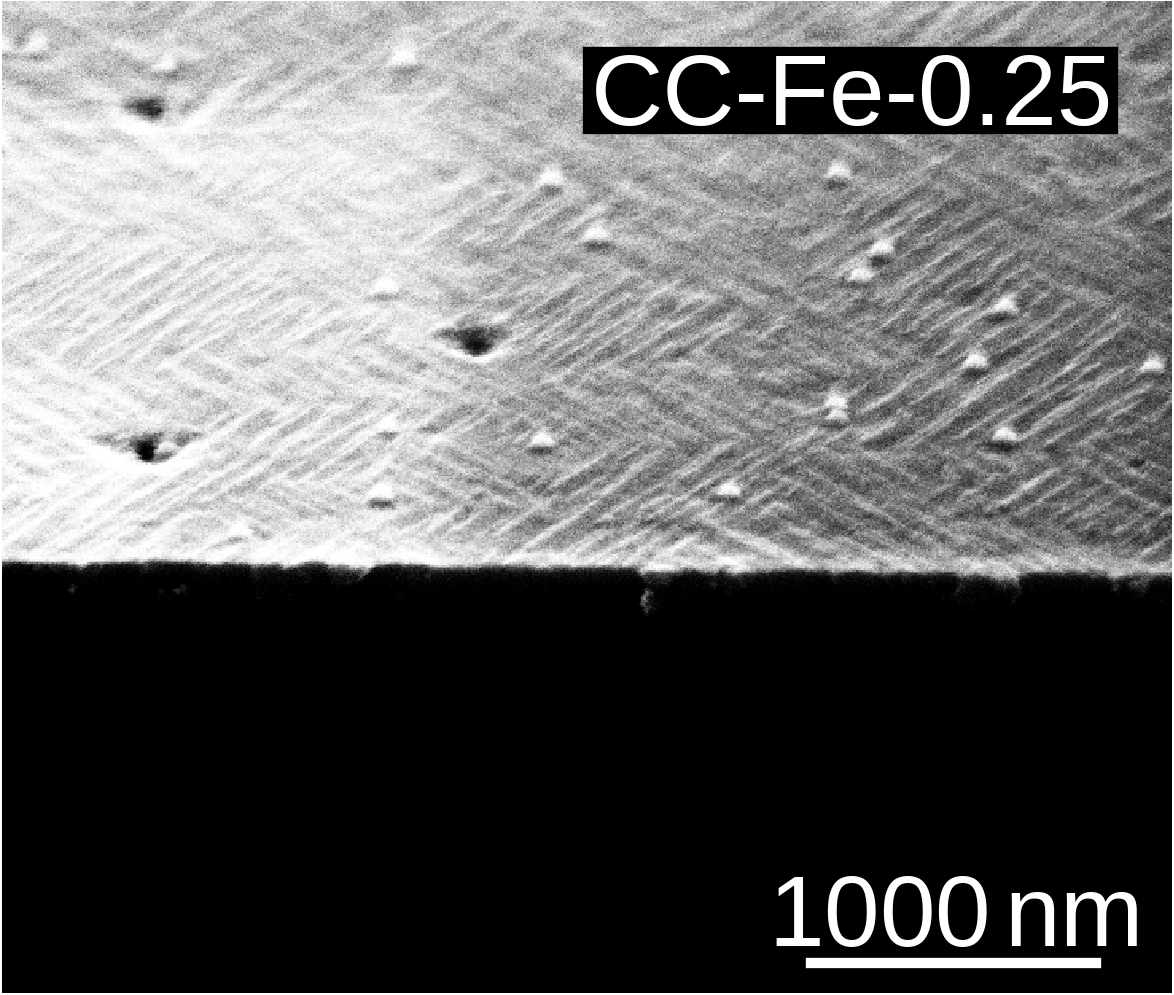
\includegraphics{colloidalCrystals_SEM_CC-Fe-0_25_xsSmallZoom}
    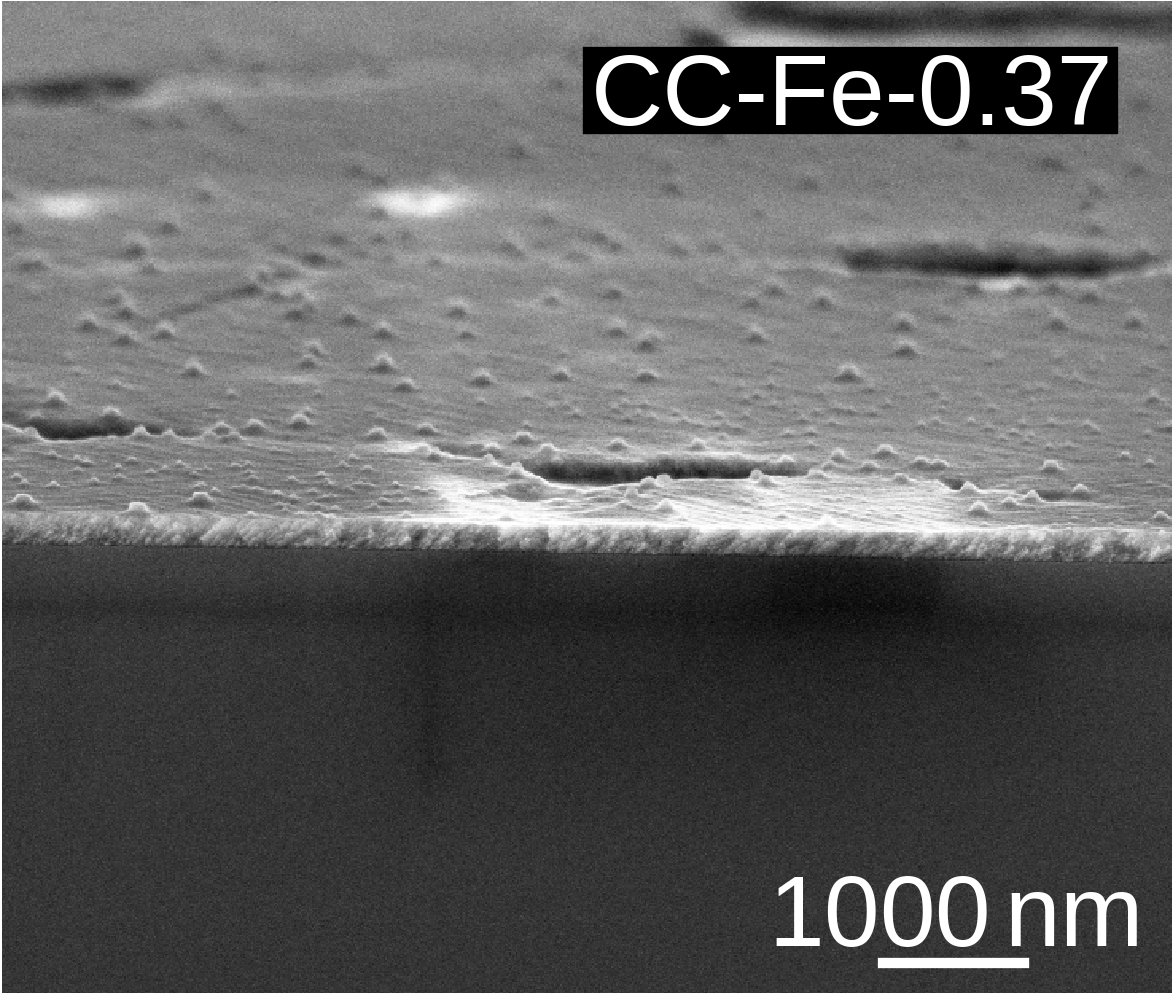
\includegraphics{colloidalCrystals_SEM_CC-Fe-0_37_xsSmallZoom}
    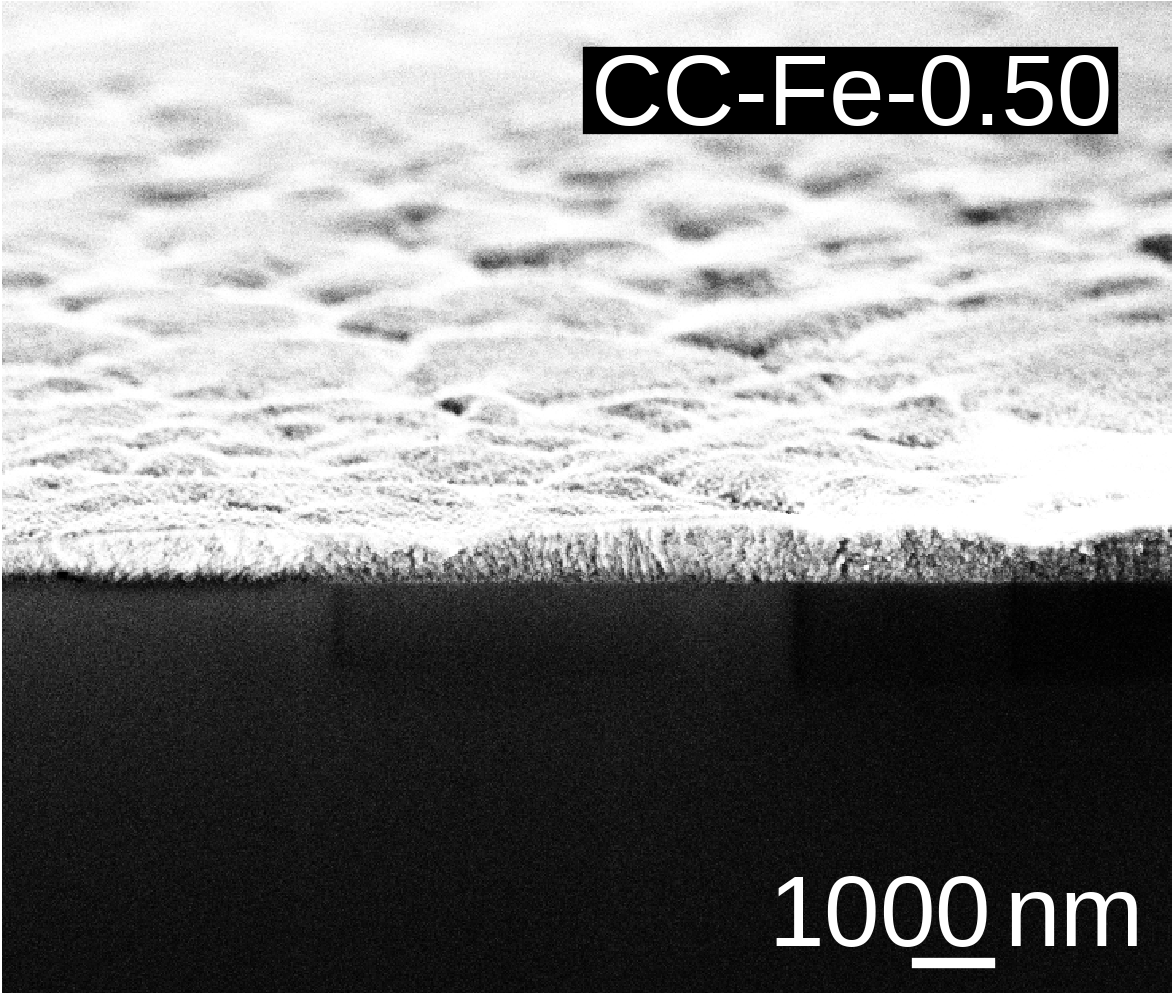
\includegraphics{colloidalCrystals_SEM_CC-Fe-0_50_xsSmallZoom}
    \caption{\label{fig:colloidalCrystals:structure:semLowMag}Cross-sectional micrographs of CC-Fe-0.25 (left), CC-Fe-0.37 (center), CC-Fe-0.50 (right) with low magnification.}
  \end{figure}

  \begin{figure}[tb]
    \centering
    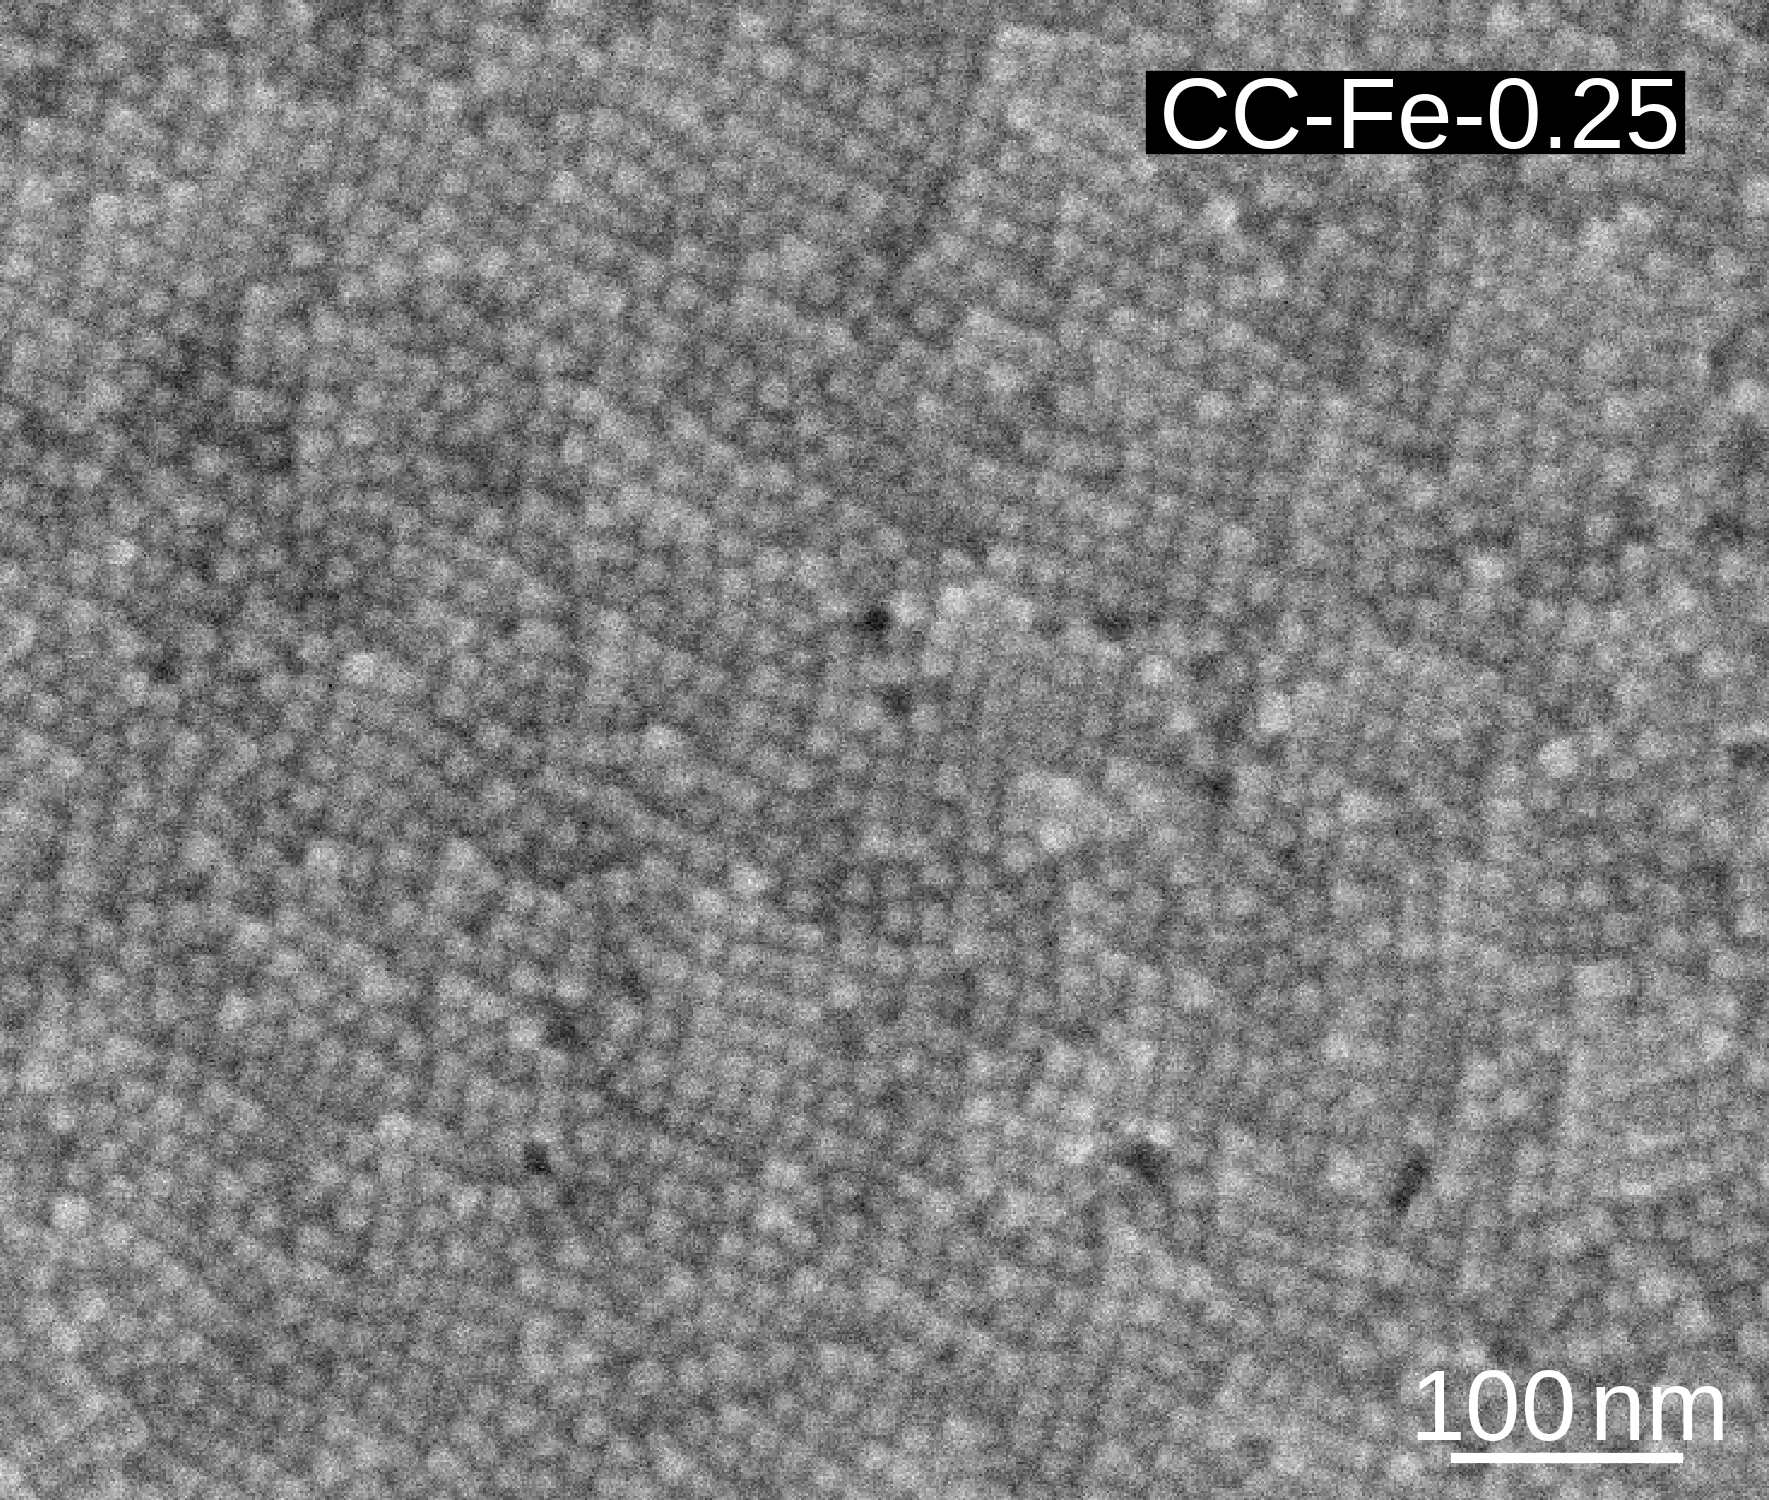
\includegraphics{colloidalCrystals_SEM_CC-Fe-0_25}
    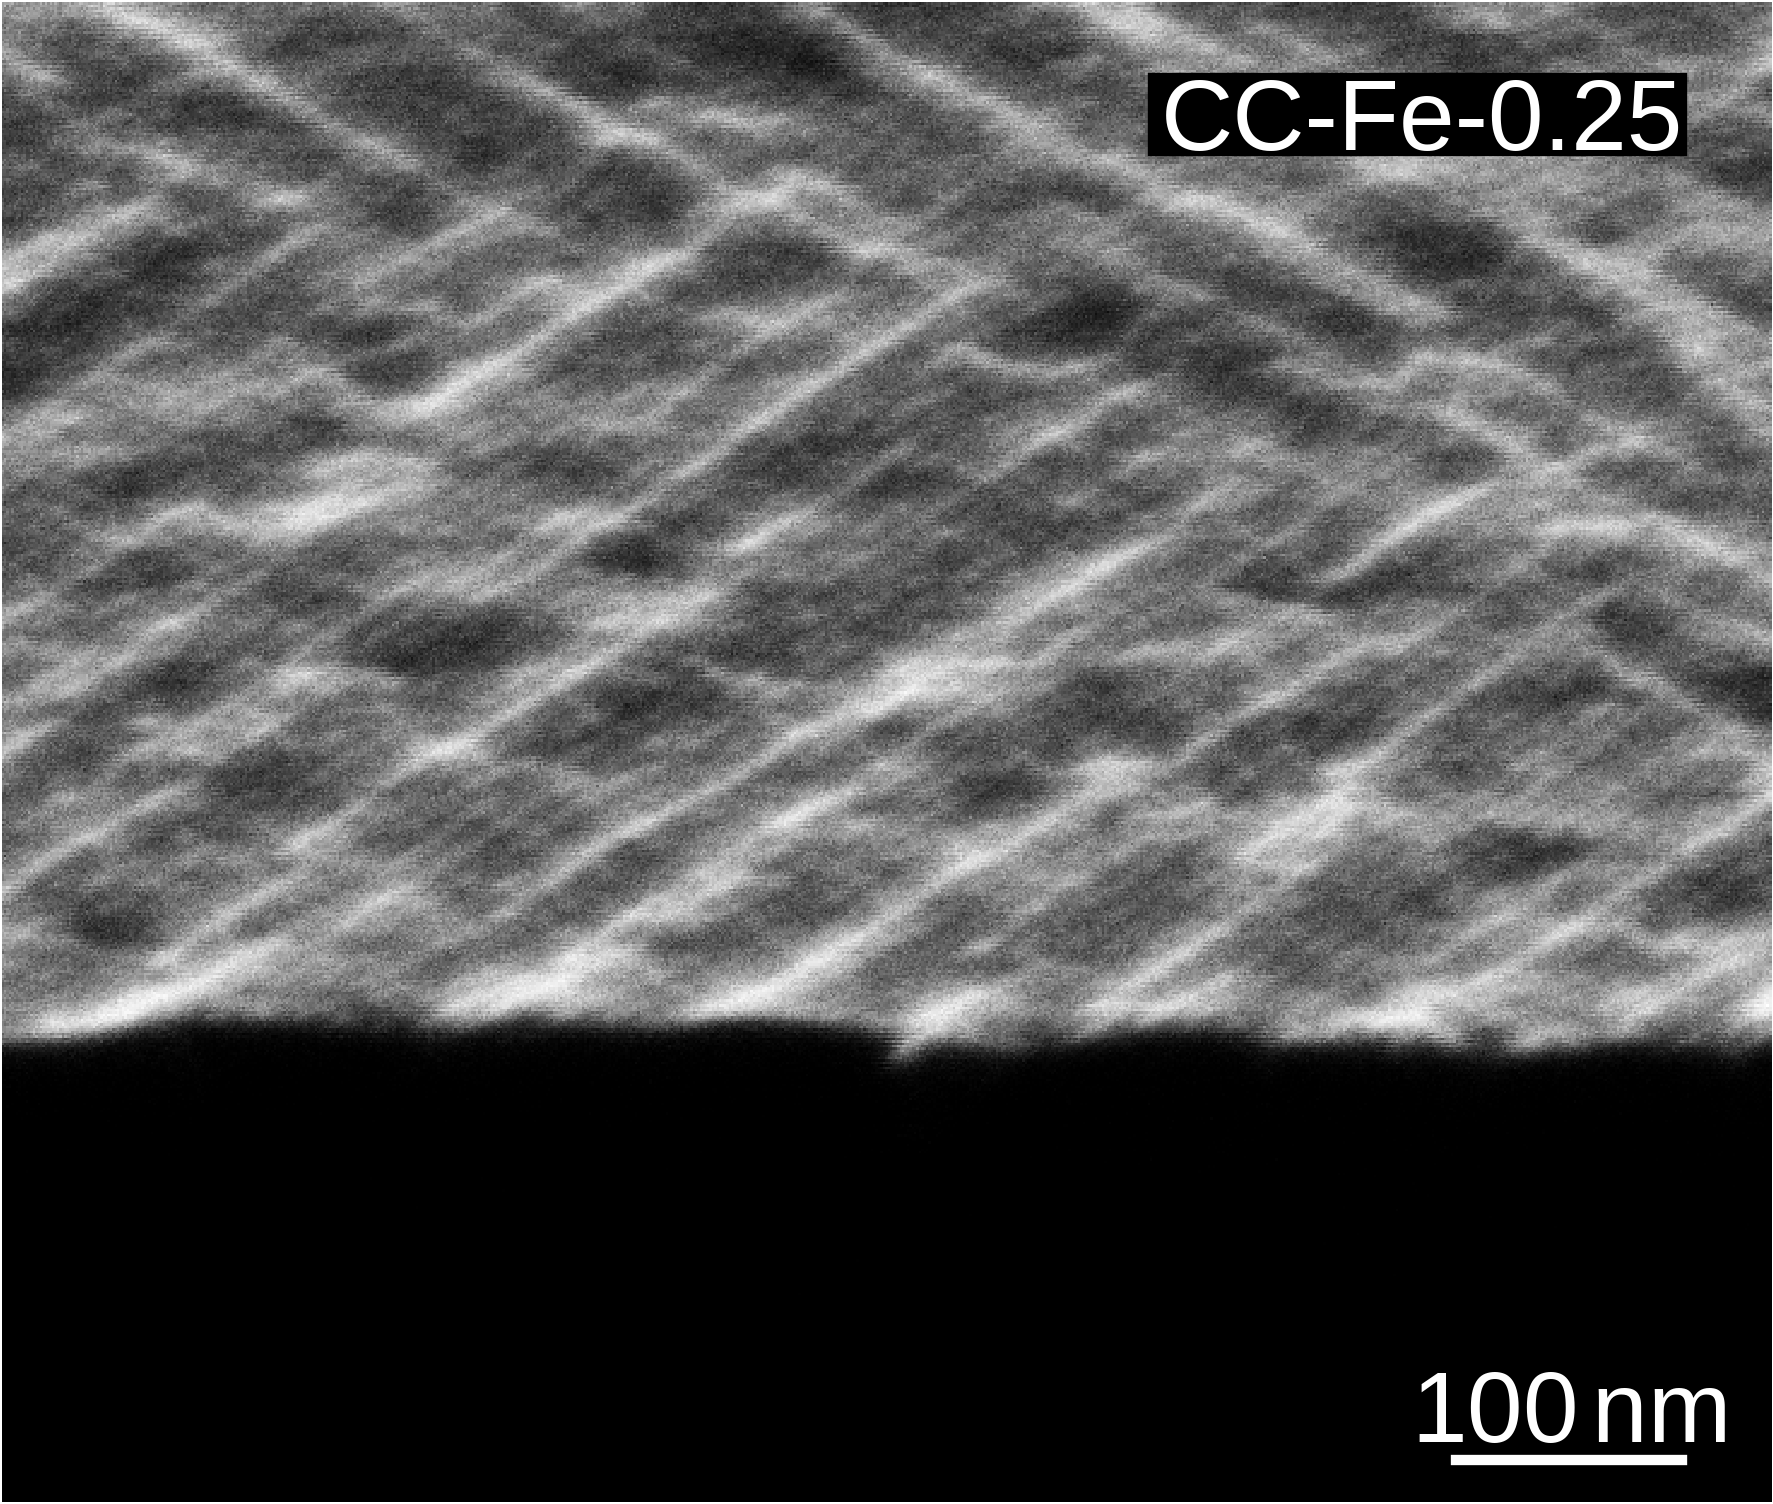
\includegraphics{colloidalCrystals_SEM_CC-Fe-0_25_xs}
    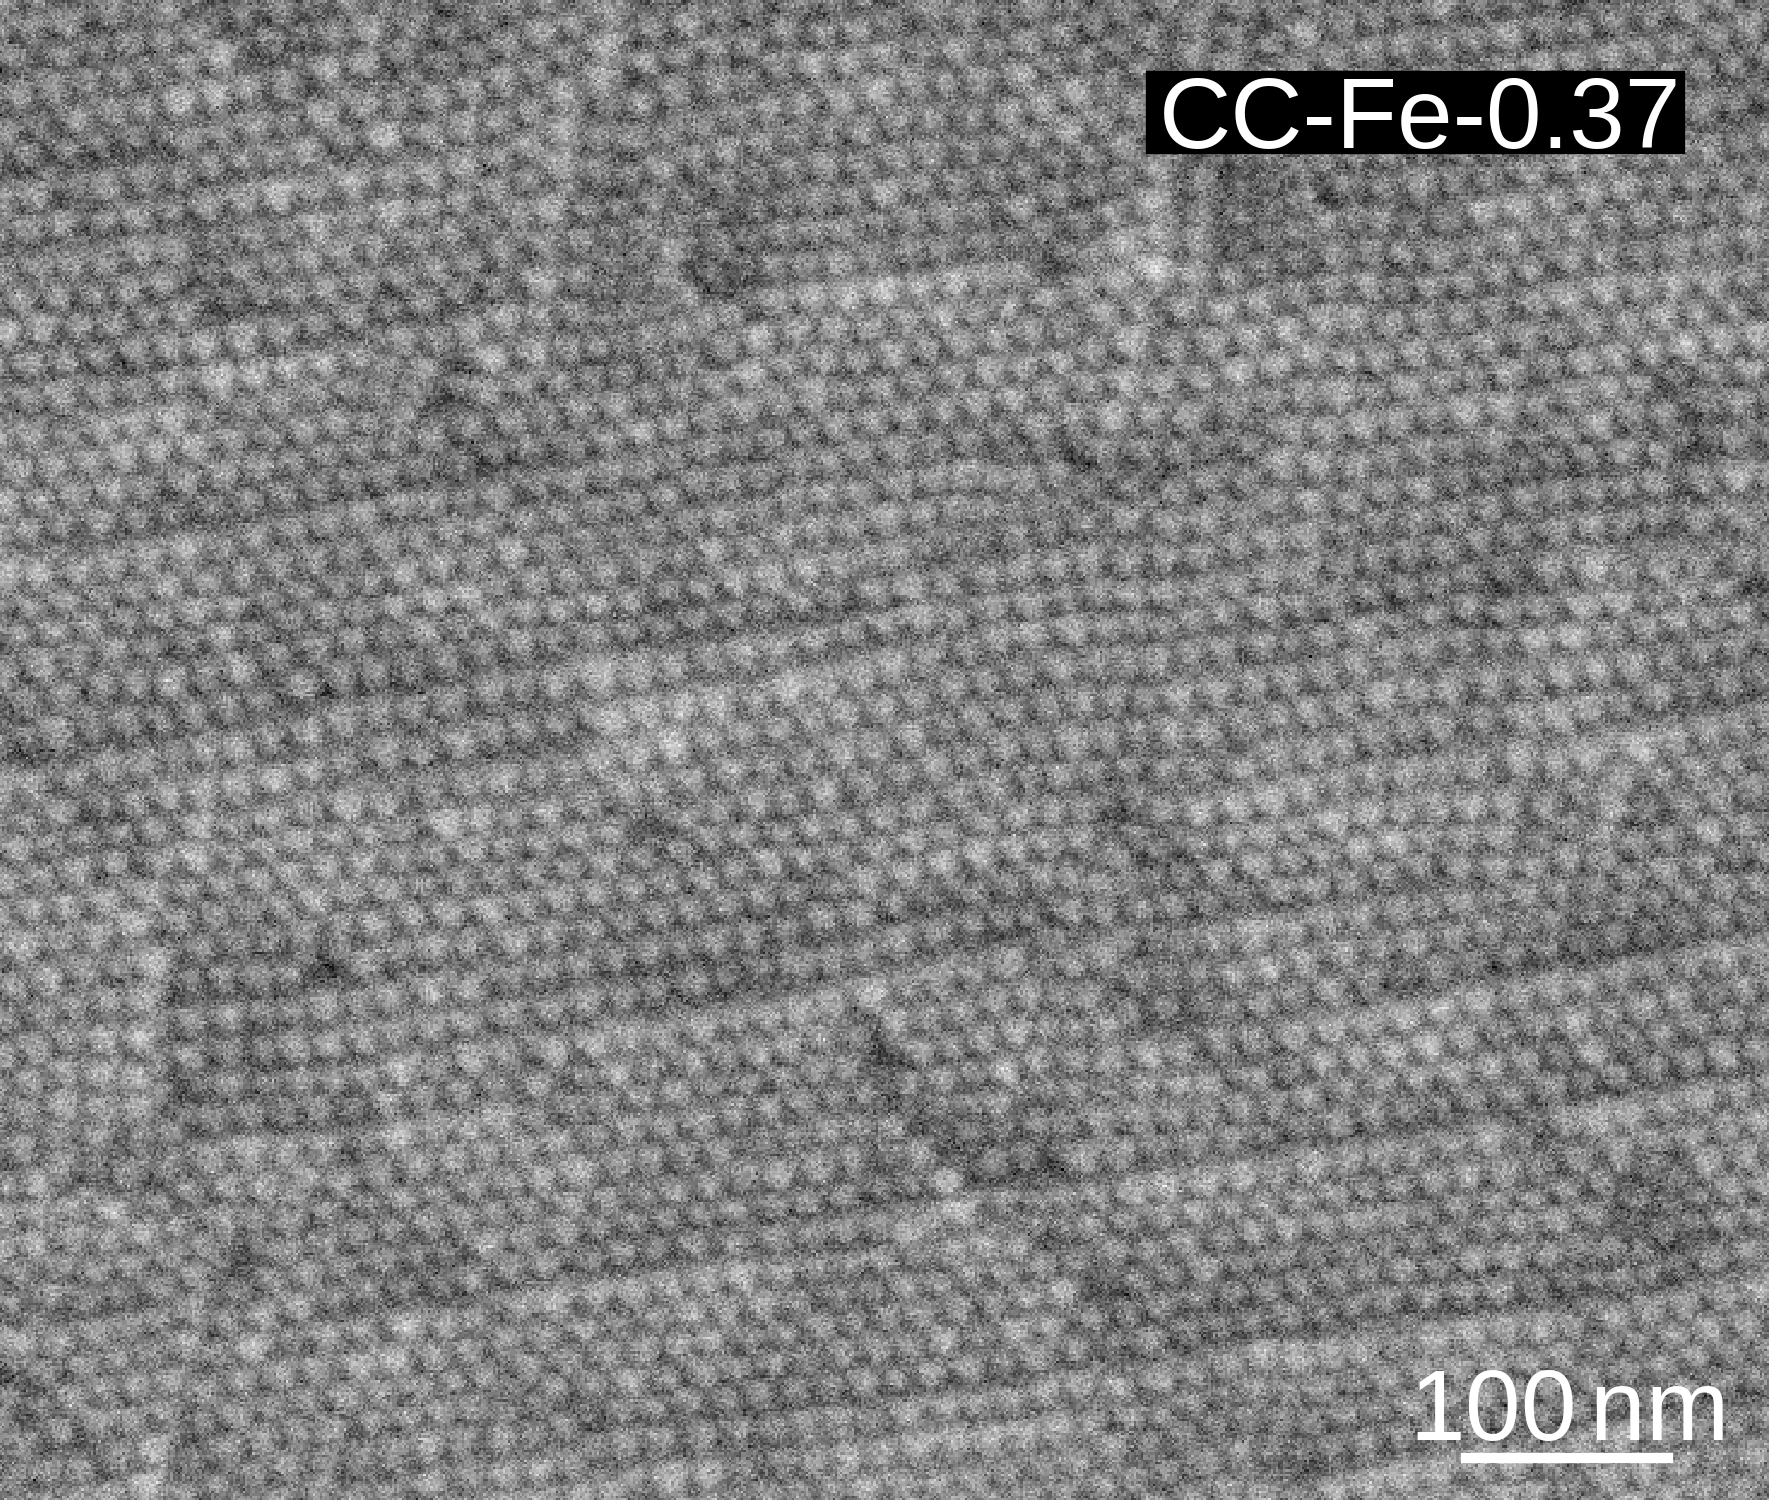
\includegraphics{colloidalCrystals_SEM_CC-Fe-0_37}
    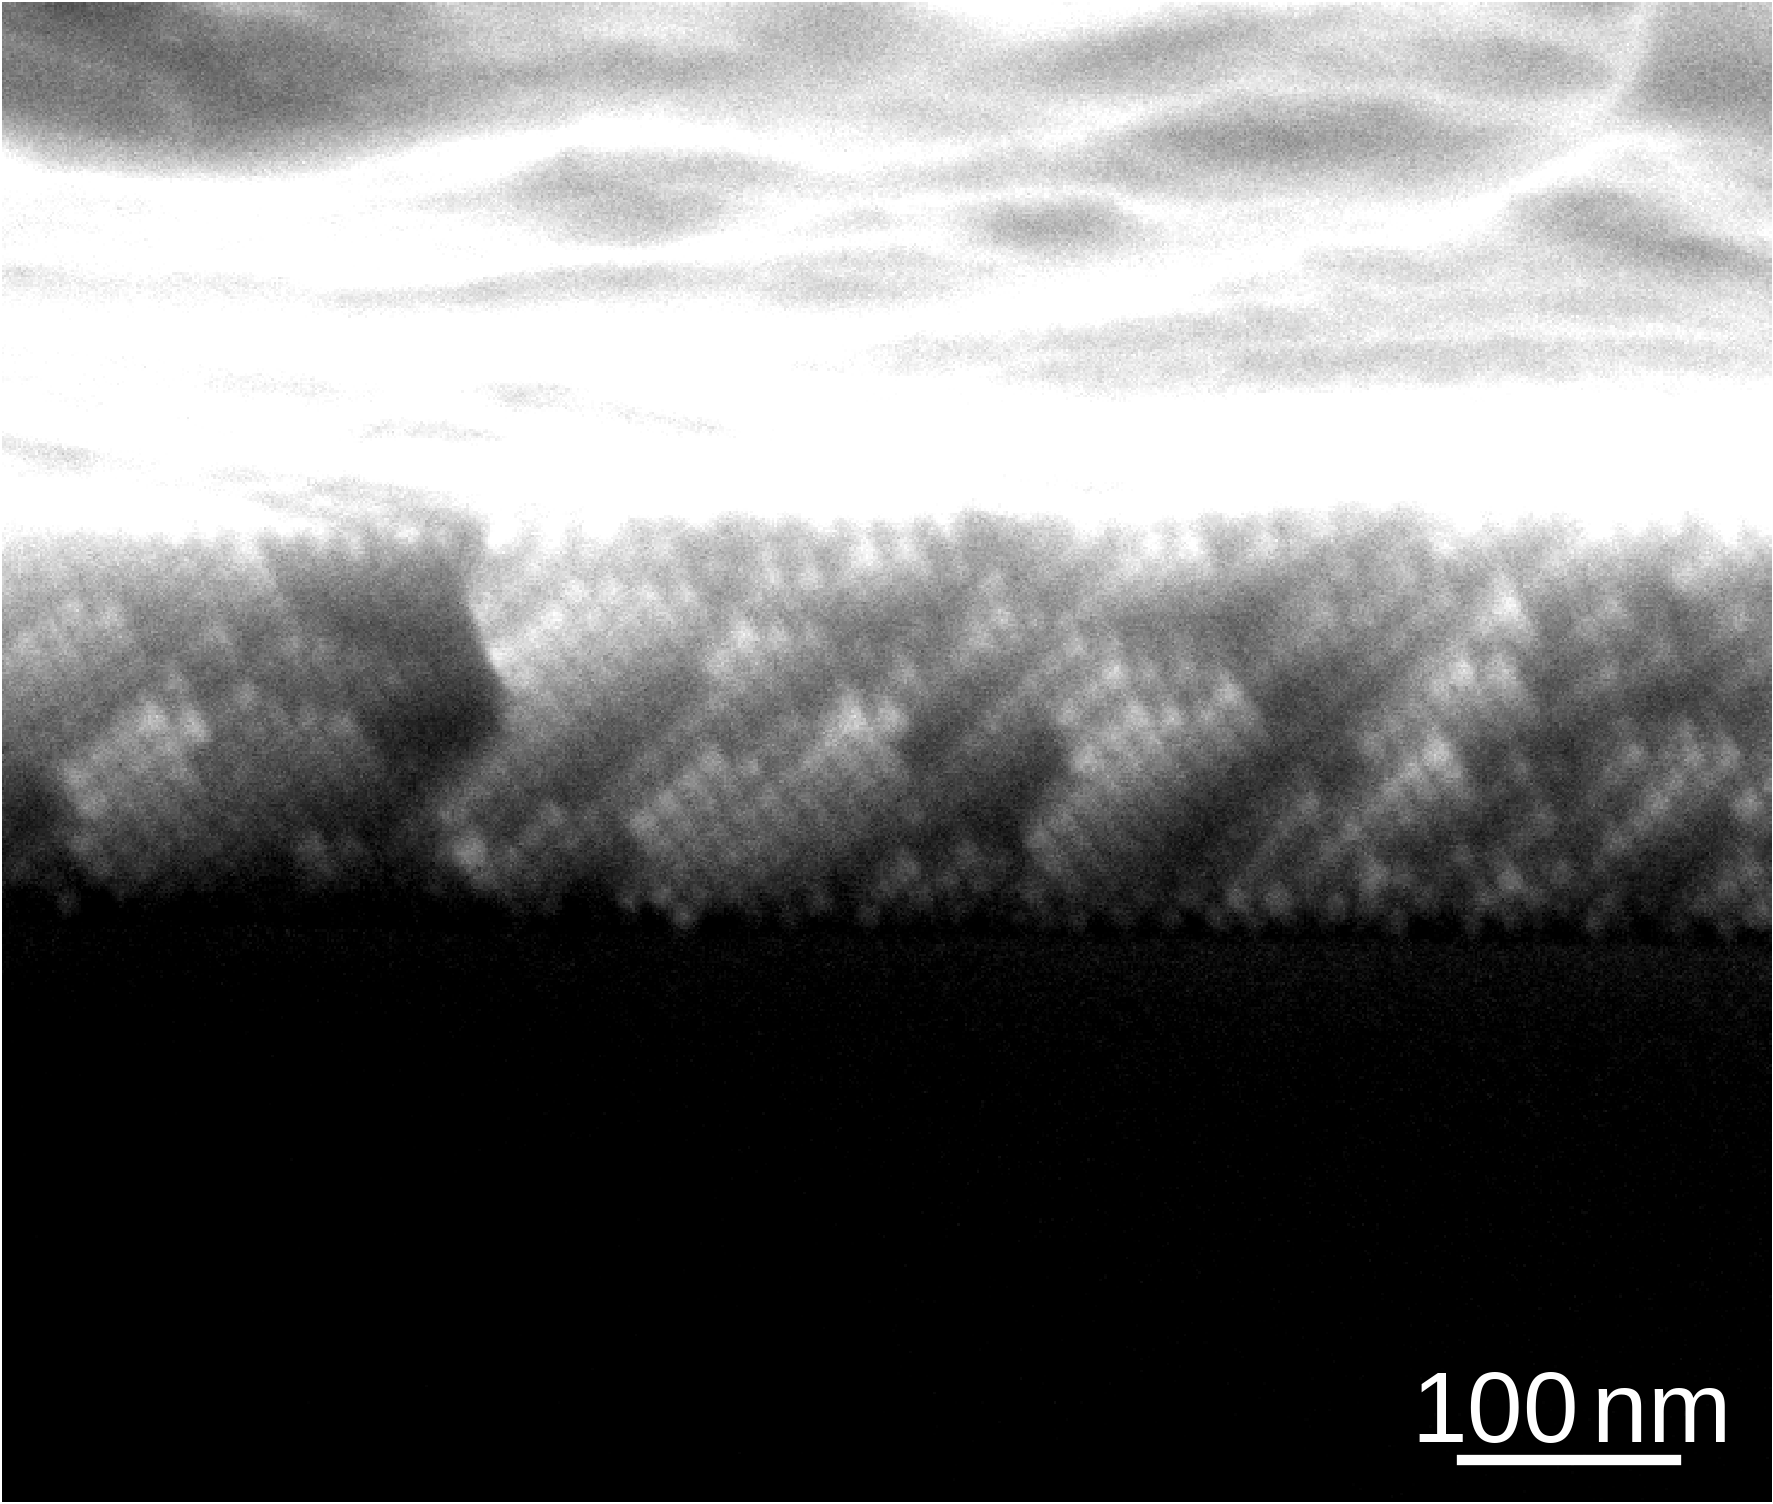
\includegraphics{colloidalCrystals_SEM_CC-Fe-0_37_xs}
    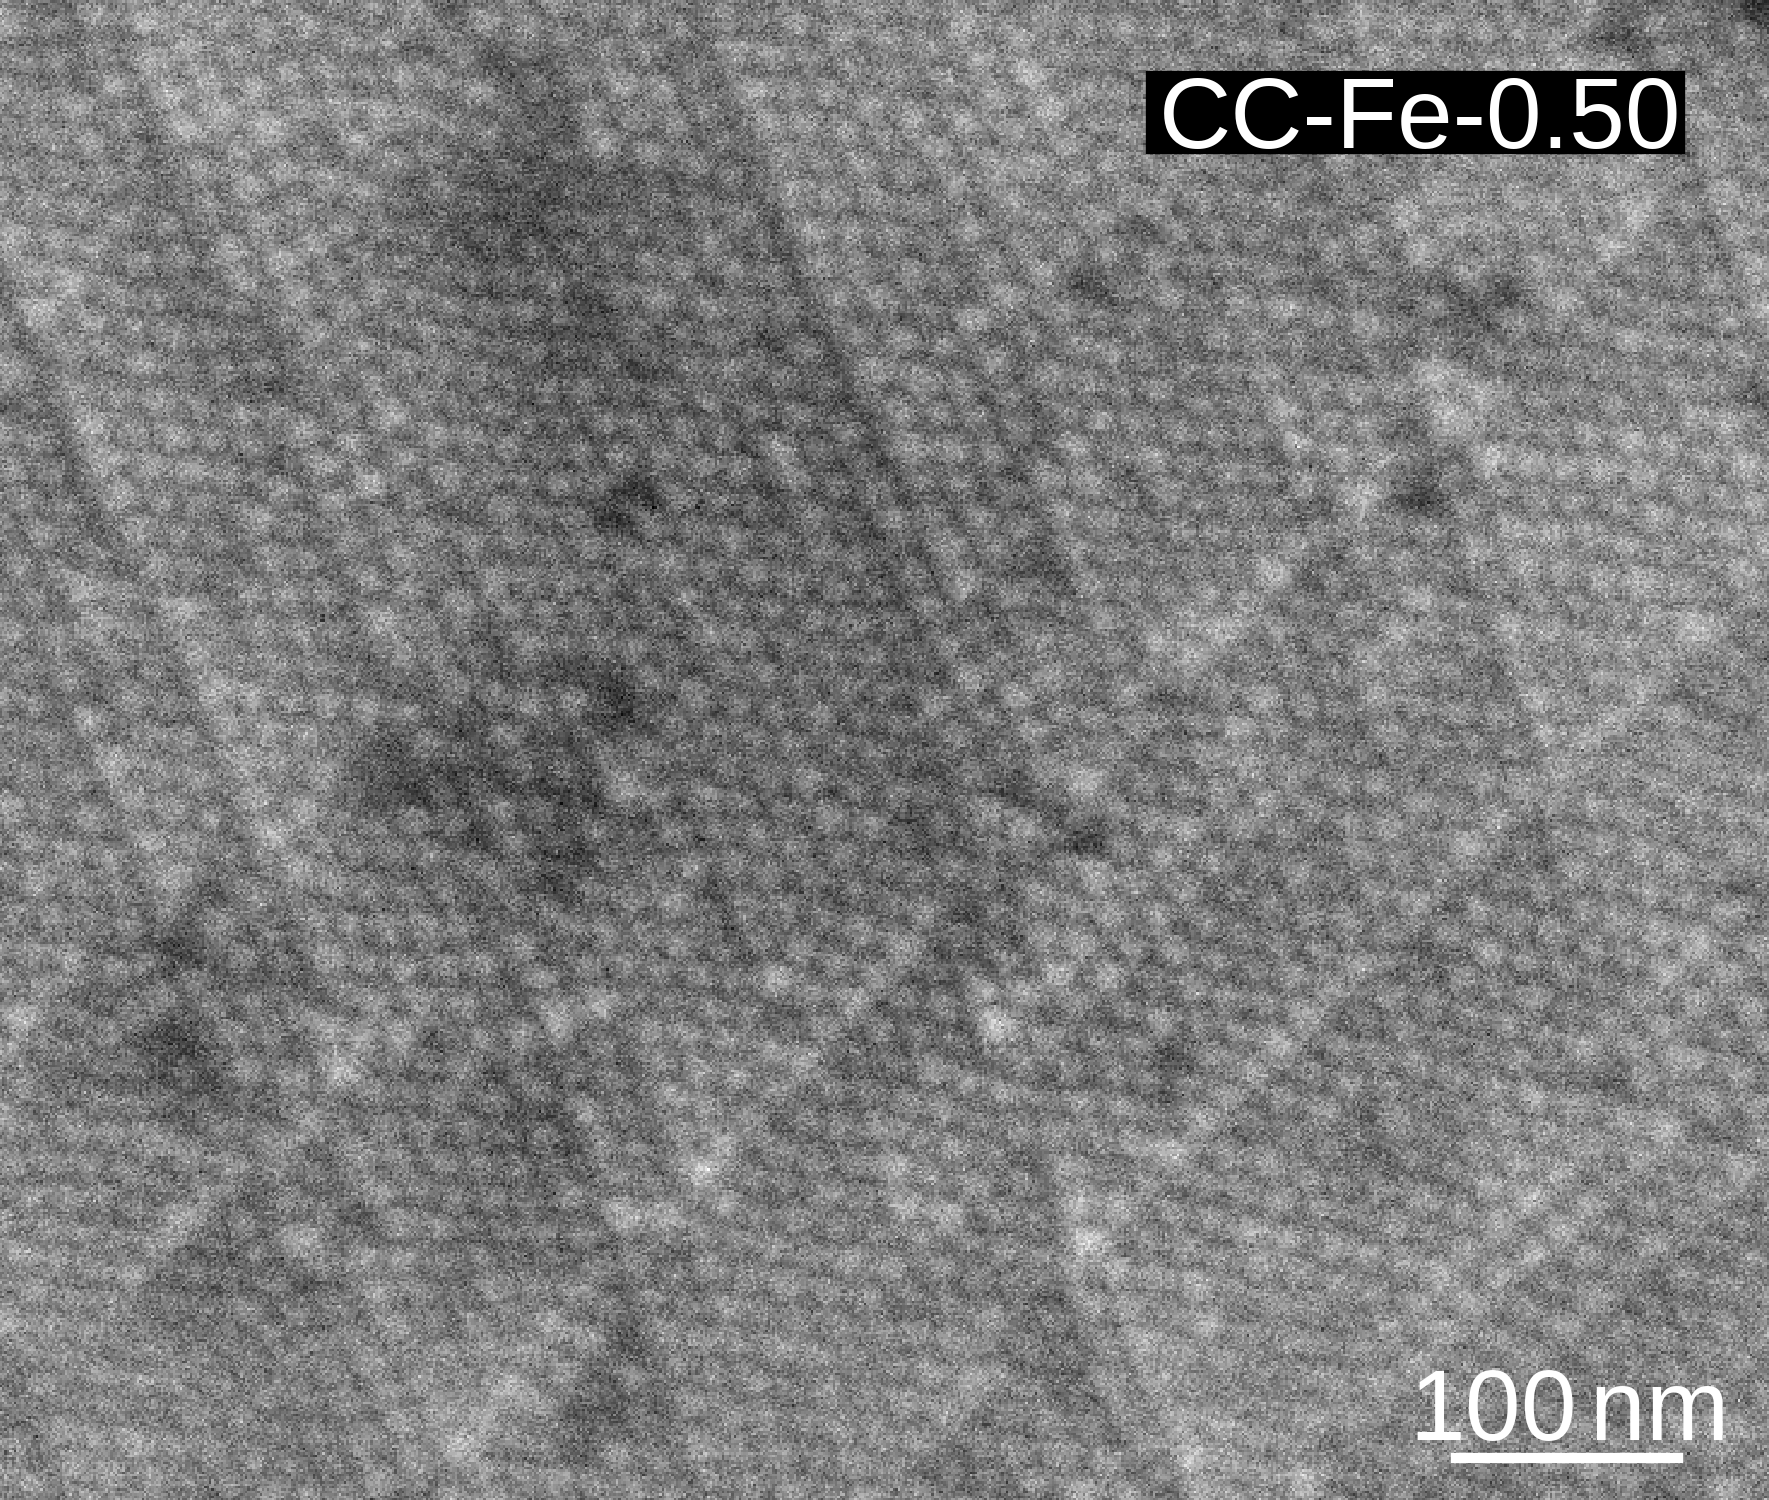
\includegraphics{colloidalCrystals_SEM_CC-Fe-0_50}
    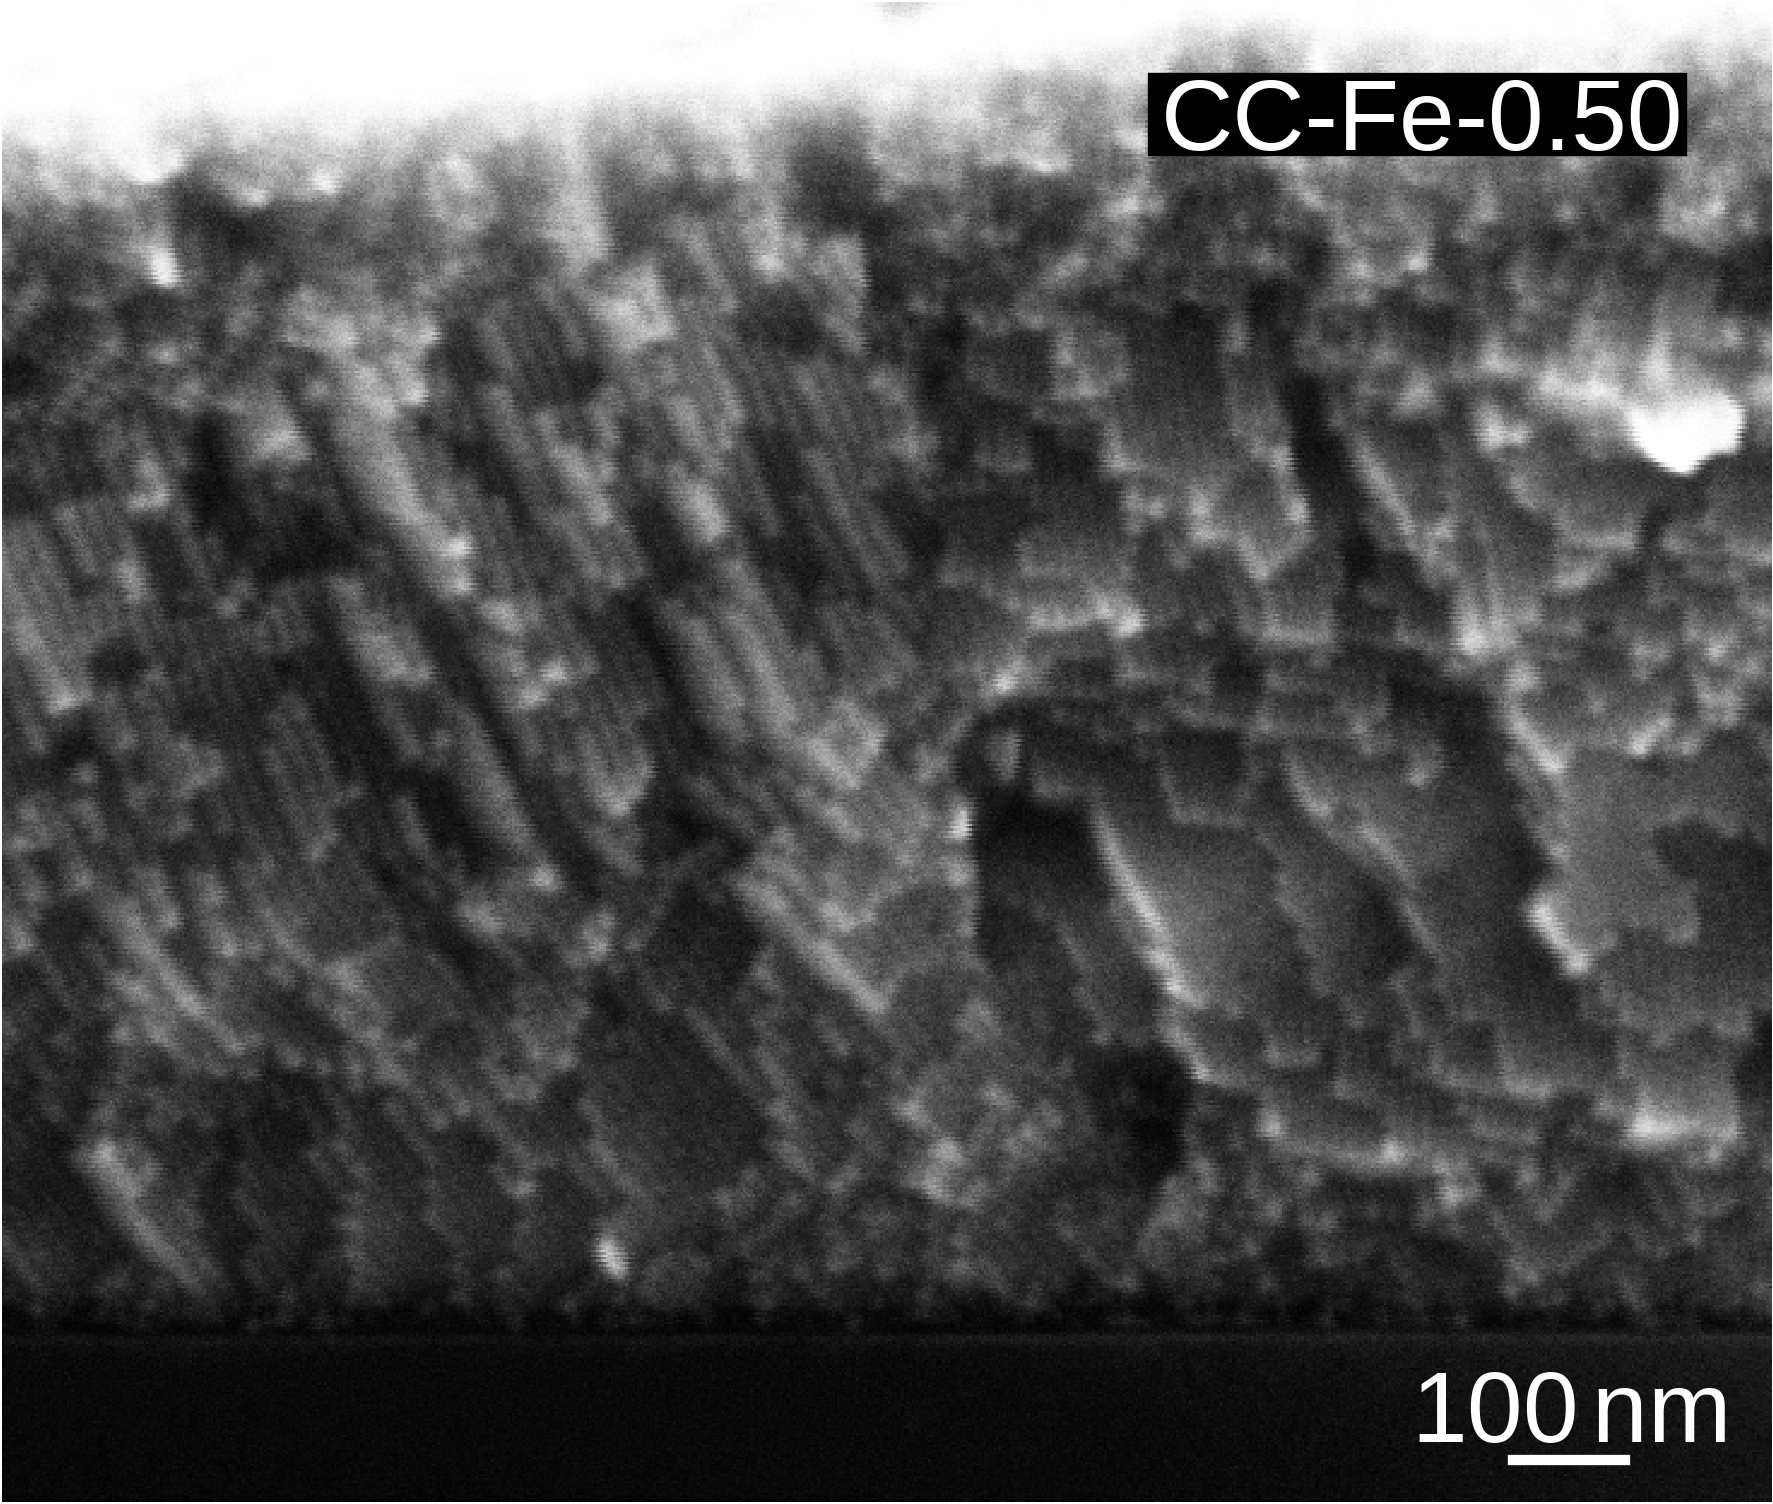
\includegraphics{colloidalCrystals_SEM_CC-Fe-0_50_xs}
    \caption{\label{fig:colloidalCrystals:structure:sem}Micrographs CC-Fe-0.25 (upper), CC-Fe-0.37 (center), CC-Fe-0.50 (lower) viewed from the top (left) and a cross-sectional view (right). }
  \end{figure}
  Using scanning electron microscopy the structure of the colloidal crystals is probed at multiple positions of the sample, where exemplary top views and cross-sectional micrographs are shown in \reffig{fig:colloidalCrystals:structure:sem}.
  The shown cross-sectional views are performed along the direction perpendicular to the drying direction near the center of the sample.
  It is visible that by variation of the nanoparticle concentration in the dispersion, the crystal thickness is non-linearly tuned.
  Where the dispersion with $0.25 \unit{mg \, mL^{-1}}$ shows only a thin layer of ordered cubes, where the thickness can not be determined due to a low contrast with the substrate, $0.37 \unit{mg \, mL^{-1}}$ shows a thickness in the order of $200 \unit{nm}$ and $0.50 \unit{mg \, mL^{-1}}$ leads to a thickness close to $1 \unit{\musf m}$.

  From lower magnification views of the cross-section, shown in \reffig{fig:colloidalCrystals:structure:semLowMag}, locally a relatively homogeneous thickness is observed for CC-Fe-0.25 and CC-Fe-0.37, but a high variation in thickness in CC-Fe-0.50.
  All samples show holes in the structure and organic remnants are visible on the surface of CC-Fe-0.25 and CC-Fe-0.37.
  Furthermore, holes in the structures are visible from the cross-sectional views.
  A possibly origin might be an incomplete wetting of the wafer surface during the vertical evaporation process, which resulted in the formation of empty spots in the structure.

  From the top view micrographs, the formation of terraces on the sample surface that stretch over several $100 \unit{nm}$ is visible.
  The best ordering in the cross-sectional view is observed for CC-Fe-0.37, where for CC-Fe-0.25 the sample is not thick enough to evaluate the vertical ordering.
  In the cross-sectional view of CC-Fe-0.37 in \reffig{fig:colloidalCrystals:structure:sem} a tilting angle of the nanocubes can be estimated from the micrographs.
  Measuring the tilt at multiple positions relative to the substrate surface yields an angle of $41(1) ^\circ$.
  For CC-Fe-0.25 the tilted lines form an angle of $32(1) ^\circ$ with respect to the horizontal breaking line and for CC-Fe-0.50 a large variation in the range of $40 - 55 ^\circ$ is visible.
  The more disordered structure of CC-Fe-0.50 could be due to the violent breaking of the thick sample that is necessary to obtain cross-sectional SEM and could have a more structure damaging effect on the thicker layer.
  Furthermore, a large thickness variation is visible in CC-Fe-0.50 in the low magnification view of \reffig{fig:colloidalCrystals:structure:semLowMag}.
  Not visible from the shown cross-sectional SEM micrographs is whether the thickness of the layers varies along the drying direction, which might be expected as the dispersion concentration increases as the solvent evaporates during the vertical deposition process.
\end{document}